\documentclass[lucida]{sp} % use if you have the Lucida LaTeX fonts
%\documentclass{sp}          % default: uses Times font
\usepackage{textcomp}
\usepackage{tikz}
\usepackage{gb4e}
\usepackage{amssymb}
\usepackage{pifont}
\usepackage{tipa}
\usetikzlibrary{fit,positioning}
\usepackage{setspace}

%tables
\usepackage{tabularx}
\usepackage{array}
\usepackage{booktabs}
\usepackage{multirow}
\newcolumntype{L}[1]{>{\raggedright\let\newline\\\arraybackslash\hspace{0pt}}m{#1}}
\newcolumntype{C}[1]{>{\centering\let\newline\\\arraybackslash\hspace{0pt}}m{#1}}
\newcolumntype{R}[1]{>{\raggedleft\let\newline\\\arraybackslash\hspace{0pt}}m{#1}}
\newcommand{\possessivecite}[1]{\citeauthor{#1}'s (\citeyear{#1})}

%=====================================================================
%========================= preamble material =========================

% Metadata for the PDF output. ASCII-only!
\pdfauthor{Sebastian Schuster}
\pdftitle{Early Marking of Oblique Noun Phrases in German and English}
%\pdfkeywords{Full keyword list}

% Optional short title inside square brackets, for the running headers.
% If no short title is given, no title appears in the headers.
\title{Early Marking of Oblique Noun Phrases \\ in German and English
 \thanks{I would like to thank my QP committee members, Beth Levin and Chris Manning, and in particular my QP chair, Eve Clark,  for their advice and valuable discussions. I would also like to thank Meghan Sumner for her advice on developing the experiment, and Ed King, Masoud Jasbi, and Simon Todd for their feedback and suggestions at various stages of this project.}}

% Optional short author inside square brackets, for the running headers.
% If no short author is given, no authors print in the headers.
\author{% As many authors as you like, each separated by \AND.
  \spauthor{Sebastian Schuster\\ \today}
}

%=====================================================================

\begin{document}

%=====================================================================
%============================ frontmatter ============================

\maketitle

\begin{abstract}

In this paper, I re-investigate the phenomenon that some English-speaking children use the preposition \textit{from} to mark standards of comparison, demoted agents, and possessors, and I evaluate whether there is cross-linguistic evidence for children making use of a conceptual category of \textsc{source} \citep{clark1989a} when formulating their early utterances. By comparing the early marking of standards of comparison in German and English through a corpus study and an elicitation task, I find that German-speaking children do not use \textit{von} (`from') to mark standards of comparison, whereas some English-speaking children mark standards of comparison with \textit{from}. Based on this result, I argue that English-speaking children overextend the conventional construction \textit{different from} rather than relying on a conceptual category of \textsc{source}.  I further present potential alternative explanations for the non-conventional uses of \textit{from} to mark demoted agents and possessors. 
\end{abstract}

%\begin{keywords}
%  Keywords (special formatting is fine)
%\end{keywords}

%=====================================================================
%============================ article text ===========================

\section{Introduction}

Grammatical prepositions such as  \textit{from}, \textit{by}, and \textit{with} can be used to mark a large number of semantic roles and their interpretation is highly context-dependent. Therefore, it is not surprising that children's early utterances sometimes contain non-conventional uses of these prepositions. What is more surprising, however, is that some of these non-conventional uses are very consistent. This is in particular true for the preposition \textit{from}. \cite{clark1989a} noted that many children acquiring English use \textit{from} to mark demoted agents (\ref{ex:child-from-agt}), possessors (\ref{ex:child-from-poss}), and standards of comparison (\ref{ex:child-from-comp}):

\begin{exe}
\ex \label{ex:child-from-agt} \begin{xlist}
\ex I took my temperature \textbf{from} the doctor. (Julia, 2;2, talking about a visit to the doctor)
\ex I was caught \textbf{from} you before. (Jessica, 5;11, during a chase-game)
\end{xlist}
\ex \label{ex:child-from-poss}  \begin{xlist}
\ex You can be a mom \textbf{from} two babies. (Damon, 3;7.5, assigning roles in a game)
\ex That's a finger \textbf{from} him (Shem, 3;7.5)
\end{xlist}
\ex \label{ex:child-from-comp} \begin{xlist}
\ex See? This ear is longer \textbf{from} the other ear. (Abe, 3;1.15, talking about a toy rabbit)
\ex Herb's the tallest \textbf{from} me and you're the tallest \textbf{from} me. (Damon, 3;7.1, comparing his height to that of his parents)
\end{xlist}
\end{exe}
Adults would have used other prepositions in all of these sentences and \cite{clark1989a} therefore argued that these uses of \textit{from} cannot be explained by the adult input. They argued that children subsume demoted agents, possessors, and standards of comparison as well as locative sources, temporal sources, and causes, under a general category of \textsc{source}, and therefore use the already aquired \textit{from} to mark all of these types of arguments. As some of these arguments are conventionally not marked with \textit{from} in English, children produce non-conventional utterances before acquiring the conventional preposition for each construction. The reasoning here is based on two observations. First, many languages extend spatial terms to non-spatial concepts and second, many languages express at least some of these arguments with the marker of locative sources. For example, within \possessivecite{palancar2002} sample of 98 languages, 30 languages use the marker of locative sources to mark demoted agents, and languages such as Uzbek and Estonian use the marker of locative sources for standards of comparison \citep{stassen1985}.  The fact that many unrelated languages appear to conflate these types of arguments is taken as evidence for a conceptual category of \textsc{source}.

To the best of my knowledge, \cite{johnson1996} is the only other work that has investigated these non-conventional uses of \textit{from}. Based on the assumption that children do not receive any form of negative feedback, he argued that children initially assign a very constrained meaning to \textit{from}. Otherwise,  if children assigned a more general meaning  such as \textsc{source} to \textit{from}, then they would subsequently have to refine their initial hypothesis, which can only happen when they receive negative feedback. He therefore suggested that children first assume that \textit{from} marks only arguments which can be simultaneously viewed as locative sources, agents, and causes, and that they later learn that \textit{from} can be used more generally, e.g., to mark locative sources independent of whether they can also be viewed as causes.
However, one of his most important assumptions, the absence of negative feedback, has been disproved since then (see, e.g., \cite{chouinard2003,hiller2016}) and therefore I will not discuss his account further in this paper. 

There is some work on the acquisition of grammatical prepositions in English: \cite{tomasello1987} investigated his daughter's first uses of prepositions and concluded that his daughter started using grammatical prepositions after she had begun to use spatial prepositions; and moreover, her first uses of grammatical prepositions were in combination with at least one other word, whereas her first uses of spatial prepositions came in the form of ``holophrases'', i.e., the entire utterance consisted only of a preposition, as in \textit{up} or \textit{out}. However, these holophrases were typically used to describe or request an action such as picking something up, and therefore his daughter's first uses of locative prepositions should probably be considered as uses of verbal particles. For this reason, it is not entirely clear whether there is a difference between the early uses of grammatical and spatial prepositions.

\cite{mckercher2001} investigated the early uses of \textit{with}. He concluded that children most likely assign a very general meaning of ``having'' to \textit{with} based on several comprehension and production experiments. This account is in many ways similar to the account by \cite{clark1989a} as both of them assume that children initially assign a single underspecified meaning to a grammatical preposition. 

More recently, \cite{kidd2008} investigated all utterances containing \textit{with} in a dense corpus from one English-speaking child. They did not find evidence for a very general meaning of \textit{with} as proposed by \cite{mckercher2001}. Instead, they concluded that the child they investigated most likely first assigned a very constrained meaning of spatial proximity to \textit{with} and then quickly progressed to a dynamic, context-dependent meaning that let him differentiate the various interpretations of \textit{with} by age 3.  

There is also more recent work on whether children possess abstract linguistic categories. For example, \cite{tomasello2000} drew upon previous results of diary studies and experiments and observed that up to age 3, children use verbs only with a very limited set of arguments that they have heard from adults. Based on this observation, he argued that young children lack abstract syntactic categories such as subject and object, as well as semantic categories such as agent and patient, because if children possessed these categories, we would expect them to be able to replace an argument with another argument of the same category and we would therefore observe many more different verb-argument combinations.

None of these more recent results necessarily contradict any of the assumptions made by the \textsc{source} account. First, neither work investigated the uses of \textit{from} and second, even if these results apply to the acquisition of \textit{from}, they mainly concern children who are younger than 3 and most children who produced non-conventional utterances with \textit{from} did so after age 3. Nevertheless, both raise the question of whether children make use of abstract conceptual categories in formulating their utterances. 

In this paper, I therefore revisit the phenomenon of children's overextensions of the preposition \textit{from} and ask whether there is cross-linguistic evidence for children relying on a conceptual category of \textsc{source} to formulate their early utterances or whether it is more likely that children overextend specific constructions. 
%Note that these two theories not only provide different explanations for the non-conventional uses of \textit{from} but also make different assumptions. Importantly, the \textsc{source} account makes the assumption that children assign a single meaning to \textit{from}, whereas if children overextend specific constructions, then we no longer have to make this assumption. 
For this purpose, I compare early uses of \textit{from} by English-speaking children to early uses of \textit{von} (`from') by German-speaking children.  As I discuss in more detail in the following section, German appears to be particularly well-suited as a language for such a comparison as it is similar to English but it differs in how \textsc{source}-type arguments are marked. 

This paper is structured as follows. I first compare how \textsc{source}-type arguments are conventionally marked in German and English (Section~\ref{sec:marking}). I then present a corpus study as well as an elicitation experiment on the early marking of standards of comparison in the two languages (Section~\ref{sec:corpus} and \ref{sec:experiment}). Finally, I present potential alternative explanations for the non-conventional marking of demoted agents and possessors (Section~\ref{sec:agents-possessors}). 

\section{Source Arguments in German and English}
\label{sec:marking}

German-speaking and English-speaking adults mark \textsc{source}-type arguments in different ways. In this section, I discuss the conventional markers for each type of argument in turn.

\subsection{Locative Sources}

Locative sources in German are conventionally introduced by the prepositions \textit{von} (`{from}') and \textit{aus} (`out of'). Both prepositions can be used to mark the source of a motion event (\ref{ex:von-locative-motion}-\ref{ex:aus-locative-motion}) as well as where an object comes from  (\ref{ex:von-locative-static}-\ref{ex:aus-locative-static})\footnote{\textit{Vom} in (\ref{ex:von-locative-motion}) and (\ref{ex:von-locative-static}) is a contraction of \textit{von} and \textit{dem}, the singular, masculine determiner in dative case.}.

\begin{exe}
\ex \label{ex:von-locative-motion} \gll Der Apfel fiel \textbf{vom} Baum. \\
The apple fell from-the.\textsc{sg}.\textsc{masc}.\textsc{dat} tree\\
`The apple fell from the tree.'

\ex \label{ex:aus-locative-motion} \gll  Sie geht \textbf{aus} dem Haus. \\
She walks out-of the house \\
`She is walking out of the house.' 

\ex \label{ex:von-locative-static} \gll Der Apfel ist \textbf{vom} Bauernhof. \\
The apple is from-the.\textsc{sg}.\textsc{masc}.\textsc{dat} farm\\
`The apple comes from the/a farm.'

\ex \label{ex:aus-locative-static} \gll das Keks \textbf{aus} der Dose \\
the cookie out-of the jar \\
`the cookie from the jar' 
\end{exe}
The difference between \textit{von} and \textit{aus} is that \textit{von} typically marks a punctual source whereas \textit{aus} is used when the source is a container or a delimited area such as a town or a country and the object used to be in the container or within the limits of that area. While this generalization holds for most conventional uses of these two prepositions, there are some exceptions to this rule. Most notably, whenever a source and a goal of a motion event are expressed in the same clause, \textit{von} tends to be used.

In English, adults also use \textit{from} and \textit{out of} to mark locative sources. \textit{Out of} is also used when the object is or was contained by the locative source. However, one contrast to German is that \textit{out of} appears to be limited to motion events and cannot be used as a modifier of a noun phrase as in (\ref{ex:out-of-locative-static}).
\begin{exe}
\ex \label{ex:out-of-locative-static} the cookie *\textbf{out of}/\textbf{from} the jar.
\end{exe}
In addition, English has a third preposition to mark locative sources, namely \textit{off (of)}, which can be used instead of \textit{from} to highlight the fact that the source is a surface.

\begin{exe}
\ex The workers jumped \textbf{off (of)} the back of the truck.
\end{exe}

\subsection{Temporal Sources}

Starting points in time and temporal sources are also conventionally introduced by \textit{von} in German and \textit{from} in English. In German, this construction can be used to indicate when an object was made/acquired/received as in (\ref{ex:von-temp-1}), to mark the starting point of a time span (\ref{ex:von-temp-2}), and in combination with \textit{an} (`{on}') to mark a starting point in time (\ref{ex:von-temp-3}).

\begin{exe}
\ex \label{ex:von-temp-1} \gll die Zeitung \textbf{von} gestern \\
the newspaper from yesterday \\
`yesterday's newspaper'
\ex \label{ex:von-temp-2} \gll \textbf{von} Montag bis Donnerstag \\
from Monday until Thursday \\
`from Monday through Thursday'
\ex \label{ex:von-temp-3} \gll \textbf{von} morgen an \\
from tomorrow on \\
`from tomorrow on/starting tomorrow'
\end{exe}
German speakers also use the preposition \textit{ab} (`starting', `from ... on') to mark starting points in time. \textit{Ab} can be used instead of \textit{von ... an} as in (\ref{ex:ab-temp-1}), and it is frequently used in the phrase \textit{ab X Jahren} (`from X years on') in board games and movie ratings to indicate a recommended age range (\ref{ex:ab-temp-2}).

\begin{exe}
\ex \label{ex:ab-temp-1} \gll \textbf{ab} nächster Woche \\
starting next week \\
`starting next week'
\ex \label{ex:ab-temp-2} \gll \textbf{ab} 3 Jahren \\
starting 3 years \\
`age 3 and older'
\end{exe}
The complements of \textit{von} can be temporal expressions as in (\ref{ex:von-temp-1}-\ref{ex:von-temp-3}) as well as prior events (\ref{ex:von-temp-4}).
\begin{exe}
\ex \label{ex:von-temp-4} \gll der Kuchen \textbf{von} meiner Geburtstagsfeier \\
the cake from my birthday-party \\
`the cake from my birthday party'
\end{exe}
English speakers use \textit{from} in a temporal sense primarily for starting points of time spans (\ref{ex:from-temp-1})  and starting points in time (\ref{ex:from-temp-2}). Further, \textit{from} can be used in combination with events that serve as starting points (\ref{ex:from-temp-3}) or the temporal reference point of an event (\ref{ex:from-temp-4}). 

\begin{exe}
\ex \label{ex:from-temp-1} She works \textbf{from}  Monday through Friday.
\ex \label{ex:from-temp-2} \textbf{from} now until four o'clock \hfill \citep{clark1989a}
\ex \label{ex:from-temp-3} \textbf{From} World War II on, their fortunes failed. \\\null \hfill \citep{clark1989a}
\ex \label{ex:from-temp-4} the cake \textbf{from} my birthday party
\end{exe}
For certain common temporal expressions such as \textit{yesterday} or \textit{last week}, English speakers conventionally use a possessive construction instead of a prepositional phrase to mark the temporal origin (\ref{ex:poss-temp-1}-\ref{ex:poss-temp-2}).
\begin{exe}
\ex \label{ex:poss-temp-1} yesterday's bread
\ex \label{ex:poss-temp-2} last week's news
\end{exe}
Lastly, English speakers also use the participial preposition \textit{starting} to mark a starting point in time.
\begin{exe}
\ex \label{ex:starting-temp-1} \textbf{Starting} tomorrow, I will exercise more.
\end{exe}

\subsection{Demoted Agents}

German speakers conventionally use \textit{von} to mark demoted agents in passive constructions.

\begin{exe}
\ex \label{ex:von-agt-1} \gll Das Buch wurde \textbf{von} Stefanie Sargnagel geschrieben. \\
The book became from Stefanie Sargnagel written \\
`The book was written by Stefanie Sargnagel.' 
\end{exe}
In English, on the other hand,  \textit{by} is used to introduce demoted agents. However, there are some exceptions to this rule. 
First, in the construction \textit{get ... from}, \textit{from} can be used to mark a locative source, which can also be viewed as an agent.
\begin{exe}
\ex She got a book \textbf{from} John.
\ex He got a hug \textbf{from} Jill.
\ex Sue got a call \textbf{from} Mel.
\end{exe} 
Further, \cite{clark1989a} noted that in some dialects of English, \textit{from} can also be used to mark natural forces.
\begin{exe}
\ex The ice cream melted \textbf{from} the sun. \hfill \cite{clark1989a}
\ex The branch \textbf{broke} from the wind. \hfill \cite{clark1989a}
\end{exe} 

\subsection{Causes}

German speakers can use three constructions to express a causal relation. First, they can use the complementizer \textit{weil} (`{because}'), which always requires a tensed clause as its complement (\ref{ex:weil-cause-1}). Second, they can use \textit{von} (`{from}') with a nominal complement to express a non-agentive, direct\footnote{See, for example, \cite{wolff2003} for a discussion of the differences between direct and indirect causes.} causal relation (\ref{ex:von-cause-1}) \citep{maienborn2015}.  Third, they can use \textit{wegen} (`{because of}') with a nominal complement to express indirect causal relations or reasons (\ref{ex:wegen-cause-1}).
\begin{exe}
\ex \label{ex:weil-cause-1}\gll Sie war müde \textbf{weil} sie lange gearbeitet hatte.\\
She was tired because she long worked had \\
`She was tired because she had worked long hours.'
\ex  \label{ex:von-cause-1} \gll Sie war müde \textbf{von} der Arbeit.\\
She was tired from work. \\
`She was tired from work.'
\ex  \label{ex:wegen-cause-1} \gll Sie fuhren \textbf{wegen} der Hitze an den See. \\
They drove because-of the heat to the lake \\
`They drove to the lake because of the heat.'
\end{exe}
Apart from these three constructions, there also exist several idiomatic expressions that can be used to express a causal relation. For example, \textit{sterben} (`to die') can be combined with a prepositional phrase headed by \textit{an} (`on') to express the cause of death.

\begin{exe}
\ex \label{ex:sterben-an-cause-1}\gll Er starb \textbf{an} einem Herzinfarkt.\\
He died on a heart-attack. \\
`He died from/of a heart attack.'
\end{exe}
The construction \textit{Das kommt von ...} (`This/that comes from ...'), which occurs particularly often in child-directed speech,  is another way of expressing cause. This construction is often used to explain a cause or reason to a child.

\begin{exe}
\ex \label{ex:kommt-von-an-cause-1}\gll Das kommt \textbf{vom} Rumschleudern [...].\\
That comes from-the.\textsc{sg}.\textsc{masc}.\textsc{dat} hurtling-around \\
`that comes from hurtling around.'  \hfill (Mother to Leo, 2;3.20)
\end{exe}
The means for expressing cause in English are very similar to the ones in German. \textit{Because} is also used to express a causal relationship between two clauses (\ref{ex:because-cause-1}), and \textit{from} and \textit{because of} are used with a nominal complement (\ref{ex:from-cause-1}-\ref{ex:because-of-cause-1}). However, causes of death are conventionally expressed with \textit{from} or \textit{of} in English (\ref{ex:die-from-cause-1}).

\begin{exe}
\ex  \label{ex:because-cause-1} She was tired \textbf{because} she had worked long hours.
\ex \label{ex:from-cause-1} She was tired \textbf{from} work.
\ex \label{ex:because-of-cause-1}They drove to the lake \textbf{because of} the heat.
\ex \label{ex:die-from-cause-1} He died \textbf{from/of} a heart attack.
\end{exe}

%\subsection{Means}

%German:
%durch

%English:
%through


\subsection{Possessors and Partitives}

German offers several means of expressing possession. The prescriptively correct means are 
the genitive case (\ref{ex:gen-poss-1}), or, for named animate possessors, the clitic \textit{-s} (\ref{ex:s-poss-1}). 
However, in spoken language, two other options for expressing possession are more common: marking 
possessors with \textit{von} (\ref{ex:von-poss-1}) and including a possessive pronoun between the possessor and the possessum (\ref{ex:pron-poss-1}).

\begin{exe}
\ex \label{ex:gen-poss-1} \gll das Fahrrad \textbf{des} \textbf{Historikers} \\
the bicycle the.\textsc{sg}.\textsc{masc}.\textsc{gen} historian.\textsc{sg}.\textsc{masc}.\textsc{gen} \\
`the historian's bicycle'
\ex \label{ex:s-poss-1} \gll Ronald\textbf{s} Fahrrad \\
Ronald's bicycle \\
`Ronald's bicycle'
\ex \label{ex:von-poss-1} \gll das Fahrrad \textbf{von} Ronald \\
the bicycle from Ronald\\
`Ronald's bicycle'
\ex \label{ex:pron-poss-1} \gll Ronald \textbf{sein} Fahrrad \\
Ronald his bicycle \\
`Ronald's bicycle'
\end{exe}
Partitive constructions are expressed using either the genitive case (\ref{ex:gen-part-1}) or \textit{von} (\ref{ex:von-part-1}). This also holds for arguments of relational nouns \citep{barker1995} as illustrated in (\ref{ex:gen-reln-1}) and (\ref{ex:von-reln-1}).
\begin{exe}
\ex \label{ex:gen-part-1} \gll einer \textbf{der} \textbf{Studierenden} \\
one the.\textsc{pl}.\textsc{masc}.\textsc{gen} students.\textsc{pl}.\textsc{masc}.\textsc{gen} \\
`one of the students'
\ex \label{ex:von-part-1} \gll einer \textbf{von} den Studierenden \\
one from the students\\
`one of the students'
\ex \label{ex:gen-reln-1} \gll die Zerstörung \textbf{der} \textbf{Stadt} \\
the destruction the.\textsc{sg}.\textsc{fem}.\textsc{gen} city.\textsc{sg}.\textsc{fem}.\textsc{gen} \\
`the destruction of the city'
\ex \label{ex:von-reln-1} \gll das Foto \textbf{von} Julia \\
the photo from Julia\\
`the photo of/from Julia'
\end{exe}
Note that the use of \textit{von} to mark locative sources, agents, possessors, and arguments of relational nouns can lead to ambiguities. The German phrase in (\ref{ex:von-reln-1}), for example, has four readings. Depending on the context, (\ref{ex:von-reln-1}) can express that the photo depicts Julia (argument of the relational noun), that Julia took the photo (agent), that Julia owns the photo (possessor), or that the speaker got the photo from Julia (locative source).

Possessors in English are either marked with the clitic \textit{'s} or the preposition \textit{of}. The former is used with animate possessors and the latter with inanimate ones. Partitive constructions as well as the arguments of relational nouns are marked with \textit{of}.
%character from the book

\subsection{Standards of Comparison}

In German, standards of comparison are conventionally marked with \textit{als} (`than', `{as}', `{when}').
\begin{exe}
\ex \label{ex:als-comp-1} \gll  Markus ist größer \textbf{als} Arthur.  \\ 
Markus is bigger than Arthur \\
`Markus is taller than Arthur.'
\end{exe}
In the case of equatives, \textit{so ... wie} (`so ... as') is used to mark the standard.
\begin{exe}
\ex \label{ex:so-wie-comp-1} \gll Das Haus ist \textbf{so} groß \textbf{wie} ein Schloss.  \\ 
The house is so big as a castle \\
`The house is as big as a castle.'
\end{exe}
However,  speakers of some German dialects also mark standards of comparison with \textit{wie} (but without \textit{so} before the adjective) in comparisons of inequality\footnote{Historically, \textit{als} used to be the equative marker and \textit{denn} the comparative marker \citep{thurmair2001}, so the use of \textit{wie} as a comparative marker could be the beginning of a similar shift in meaning.}. 

\begin{exe}
\ex \label{ex:wie-comp-1} \gll Sein Bruder ist kleiner \textbf{wie} er.  \\ 
His brother is smaller as he \\
`His brother is smaller than him.'
\end{exe}
Apart from \textit{als} and \textit{wie}, many adults also use the archaic preposition \textit{denn} in the fixed construction \textit{X denn je} (`X than ever'), e.g., \textit{mehr denn je} (`more than ever').

In English, standards of comparison are marked with \textit{than} as in the translation of (\ref{ex:als-comp-1}). One exception to this rule is the adjective \textit{different}, which is most often used with \textit{from}, sometimes with \textit{than}, and occasionally with \textit{to}\footnote{Among the 20,449 uses of \textit{different} with a standard of comparison in the Corpus of Contemporary American English (COCA), 75\% mark the standard with \textit{from}, 22\% with \textit{than}, and 2\% with \textit{to}.}. Equatives are marked with \textit{as ... as} (\ref{ex:as-as-comp-1}).
\begin{exe}
\ex  \label{ex:as-as-comp-1} The house is \textbf{as} big \textbf{as} a castle.
\end{exe}


%\subsection{Instruments}

%Instruments are marked with \textit{mit} (`{with}') in German.

%\begin{exe}
%\ex \label{ex:mit-instr-1} \gll  Anna schneidet den Apfel \textbf{mit} einem Messer.  \\ 
%Anna cuts the apple with a knife \\
%`Anna is cutting the apple with a knife.'
%\end{exe}
%In English, the preposition \textit{with} is predominantly used to marks instruments. 
%However, in the absence of an agent, instruments that can appear in subject position are marked with \textit{by} \citep{schlesinger1989}.

%\begin{exe}
%\ex The horse was hit \textbf{by} the stick.
%\end{exe} 

%\subsection{Cessation}



%- abhalten von
%- verhindern dass
%- jmd. davon abhalten, etwas zu tun
%- jmd. an X hindern

%English
%- stop sb from doing something
%- prevent sb from 
%- keep sb from 




%\subsection{Accompaniment}

%german:
%mit

%english with


%\section{Other uses of these prepositions }

%- 

%
%TODO
%
%\subsection{German}
%
%\paragraph{von}
%- klug/dumm von
%
%\paragraph{aus}
%- particle
%
%- material
%
%- idioms: 
% aus dem Weg,
%  we ran out of something
%
%\paragraph{ab}
%
%
%- verbal prefix
%
%The prefix "ab-" usually - but not always - carries the notion of "away from". Some of the many possibilities:
% (abschreiben, abfahren, abholzen, abbrechen, abnehmen, abfliegen, abriegeln, abhören, abkommen, abfahren, abstimmen, abtreiben, abnutzen, ablenken)
%
%\paragraph{als}
%- when I was 15...
%
%- as (Ich verkleide mich als...)
%
%- als ob es etwas Neues gewesen wäre!
%
%\paragraph{mit}
%
%- comitative with
%- attributive with
%- manner
%- reference (Kannst du mir mit dem Problem helfen?)
%- material (ich hab das mit den steinen gebaut)
%
%\subsection{English}
%\paragraph{from}
%
%- change of states
%
%- additional causes/reasons: from the look on his face, ...
%
%\paragraph{out}
%
%-adverb/adjective
%
%- light is out
%- outside
%- out!
%- we're out (of...)
%- 
%
%
%
%\paragraph{off}
%
%- out of operation
%- You are off on that point. (you are wrong)
%- This button is about to come off
%- The agreement is off.
%- The electricity is off.
%
%\paragraph{by}
%- proximity
%- means: she arrived by air
%- no later than: I'm done by 5 o'clock.
%
%\paragraph{than}
%- only used for comparatives
%\paragraph{with}
%
% (\cite[Ch. 2]{mckercher2001})
%- comitative with
%- attributive with
%- manner
%- reference (Kannst du mir mit dem Problem helfen?)
%- proximity You left your keys with your wallet
%- cause: the man was paralyzed with fear (\cite{mckercher2001})
%- material (i built the house with blocks)

\subsection{Summary}

Table~\ref{tbl:prep-summary} summarizes which prepositions and other case-marking mechanisms are conventionally used to mark \textsc{source} arguments. As this this table shows, standard of comparison is the only \textsc{source} argument that is never marked with \textit{von} in German. In English, demoted agents, possessors and partitives are never marked with \textit{from}.

\begin{table}
\begin{tabularx}{\textwidth}{l | c | c}
& \textbf{German} & \textbf{English} \\ \midrule
Locative sources & \textit{von}, \textit{aus} &\ \textit{from}, \textit{out of}, \textit{off of} \ \\ \hline
Temporal sources & \textit{von}, \textit{ab} & \textit{from}, \textit{'s}, \textit{starting} \\ \hline
Demoted agents & \textit{von} & \textit{by}, (\textit{from}) \\ \hline
Natural forces & \textit{von} & \textit{by}, \textit{from} \\ \hline
\multirow{2}{*}{Causes} &\  \textit{von}, \textit{weil},  \  & \textit{from}, \textit{because}, \\
& \textit{wegen}, (\textit{an}) & \textit{because of}, (\textit{of})  \\ \hline
\multirow{2}{*}{Possessors \& partitives} & {genitive, \textit{-s}, \textit{von}, } &  \multirow{2}{*}{\textit{'s}, \textit{of}  } \\ 
& possessive pronoun & \\ \hline
\multirow{2}{*}{Standards of comparison} \ \ \ & \textit{als}, \textit{so ... wie}, & \textit{than}, \textit{as ... as},  \\
&  (\textit{denn}), (\textit{wie}) & (\textit{from}) \\
\end{tabularx}
\caption{Summary of the conventional means for marking \textsc{source} arguments in German and English. Parentheses indicate non-standard uses or that the preposition can only be used in special contexts.}\label{tbl:prep-summary}
\end{table}

\section{Corpus Study}
\label{sec:corpus}

As discussed in the previous section, standard of comparison (\textsc{comparison}) is the only type of argument never marked with \textit{von} in German. At the same time, English speakers mark \textsc{comparison} in some cases with \textit{from}. For this reason, the means that German-speaking children use to express \textsc{comparison} could provide additional evidence for a conceptual category of \textsc{source} or could suggest that the non-conventional uses are limited to English-speaking children and are therefore language-dependent.

We know from \cite{clark1989a} that English-speaking children occasionally use \textit{from} to mark \textsc{comparison} in a non-conventional manner. \cite{clark1989a} attributed these non-conventional uses to children perceiving standards of comparison as abstract locative sources and therefore marking them with \textit{from}. This argument is based on \cite{jackendoff1983}, who argued that comparison can be perceived as an abstract movement away from the standard of comparison\footnote{Alternatively, one can also perceive the standard of comparison as the viewpoint of the comparison, e.g., \textit{an elephant is taller than a mouse} can be perceived as an elephant being taller from the viewpoint of a mouse. This is also reflected in the etymology of \textit{than} and \textit{denn}, which both go back to the gothic \textit{\textthorn ana},  \textit{\textthorn an}, which in return can be traced back to the ablative of the demonstrative root \textit{\textthorn a-} \citep{vonstuckrad1957, thurmair2001}.}. 
 Crucially, this explanation implies that children's non-conventional uses are independent of the linguistic input. If this is the case, some German-speaking children should also mark \textsc{comparison} with \textit{von} despite the fact that adults never use such a construction. \hfill (\textsc{Source~Hypothesis})

On the other hand, if German-speaking children never use \textit{von} to mark standards of comparison, then this suggests that the non-conventional uses in English depend on the linguistic input and that most likely some English-speaking children overextend the construction \textit{different from} to other comparative adjectives\footnote{This explanation was also suggested by \cite{johnson1996}, but he did not present any evidence for this hypothesis.}.{~\hfill(\textsc{Construction~Hypothesis})}

These  competing hypotheses make different predictions. According to the \textsc{Source Hypothesis}, as many German-speaking children should mark standards of comparison with \textit{von} as English-speaking children mark \textsc{comparison} with \textit{from} because their production of this construction should be independent of the adult input.

According to the \textsc{construction hypothesis}, German-speaking children should mark standards of comparison with \textit{von} less often than English-speaking children mark  \textsc{comparison} with \textit{from} because the marking of \textsc{comparison} with \textit{von} in the German input is never found, whereas \textsc{comparison} is occasionally marked with \textit{from} in the English input.

In order to the test these predictions, I investigated children's uses of \textit{von} and \textit{from} as well as \textit{als} and \textit{than} in several longitudinal corpora for German and English in the CHILDES Archive \citep{macwhinney2000}.

\subsection{Data}

\begin{table}
\begin{tabularx}{\textwidth}{l | c | c | c | c | c }
Corpus \ \ \ \ \ \ \ & \ \ \ Age \ \ \ & Child utterances & \  \textit{von}    \ & \   \textit{vom} \ & \  \textit{als} \  \\ \hline
Leo & 1;11.12 - 4;11.05& 190,339 & 1,152 & 111 & 331\\
Cosima & 0;00.13 - 7;02.22 & 26,138 & 148 & 29 & 60 \\
Pauline & 0;00.12 - 7;11.03 & 25,682 & 253 & 37 & 61\\
Sebastian & 0;00.17 - 7;05.11 & 24,425 & 221 & 64 & 65\\
Caroline &0;10.01 - 4;03.18& 24,982 & 90 & 26 & 22 \\
Simone & 1;09.11 - 4;00.06 & 35,107 & 97 & 16 & 16 \\
\end{tabularx}
\caption{Summary statistics of the investigated German corpora. \textit{von}, \textit{vom}, and \textit{als} denote the number of child utterances containing the relevant preposition.}\label{tbl:corpus-stats-de}
\end{table}

I used the following six German corpora for my study. Table~\ref{tbl:corpus-stats-de} contains the summary statistics for each corpus.


\paragraph{Leo}
The first corpus is a  dense longitudinal corpus, collected by \cite{behrens2006}, in the late 1990s and early 2000s. The corpus contains the transcripts of recordings of a child interacting with his parents and occasionally a research assistant at home. Between age 1;11.12 and 2;11.29, five hour-long sessions were recorded per week and supplemented with daily parental diary data noting the 10 to 30 most innovative and complex utterances of the child. Between age, 3;0 and 3;11, five hour-long sessions were recorded in every 4th week. Most of the recordings were made while Leo was playing with one of his caretakers.
\paragraph{Cosima, Pauline, and Sebastian}
The Cosima, Pauline, and Sebastian corpora were collected by Rosemarie Rigol in the 1990s. All three children were recorded for 30 minutes approximately every two weeks until age 4 and approximately every 4 weeks after that\footnote{Pauline was recorded in less regular intervals but still at least once a month during almost the entire period.}. During the recording sessions, the children mainly interacted with Ms. Rigol, the investigator, but a parent, a sibling, or a friend of the child was also often present.

\paragraph{Caroline}
The Caroline corpus was collected by Christiane von Stutterheim in the late 1980s and early 1990s. The corpus is dense for the age range between 1;9 and 2;10 with an average of 14 recordings per month but after age 2;10, there are only 6 more recordings in total up to age 4;3. The recordings were made at home while the child was interacting with her parents or playing by herself.

\paragraph{Simone}
The Simone corpus was collected by Max \cite{miller1979} (the father) in the early 1970s. The length of recordings varies  throughout the course of the study. \cite{miller1979} recorded Simone every six weeks for at least six hours. In between these six-week intervals, he made three additional shorter recordings (about one hour long). The recordings were made at home while Simone was interacting with her father and sometimes with her mother.


\vspace{1em}


%parents uses different from
%adam: y
%sarah: y
%eve: y
%shem: y
%abe: y
%naomi: n

I also investigated the use of \textit{from} and \textit{than} in the following six English corpora\footnote{These are the same corpora as used by \cite{clark1989a}.}. 
  The summary statistics of the English corpora are presented in Table~\ref{tbl:corpus-stats-en}. Additionally, I also considered the diary data on Damon for my analyses. However, as his data are not available through the CHILDES archive, I relied on the numbers reported by \cite{clark1989a}.

\begin{table}
\begin{tabularx}{\textwidth}{l | c | c | c | c  }
Corpus \ \ \ \ \ \ \ & \ \ \ Age \ \ \ & Child utterances & \  \textit{from} \   \ & \   \textit{than} \\ \hline
Adam & 2;03.04 - 5;02.12& 46,743 & 142  & 23\\
Sarah & 2;03.05 - 5;01.06 & 38,096 & 62 & 10 \\
Eve & 1;06.00 - 2;03.00 & 12,113 & 19 & 1\\
Shem & 2;02.16 - 3;02.02 & 18,166 & 60 & 0\\
Abe &2;04.24 - 5;00.11& 22,932 & 119 & 68 \\
Naomi & 1;02.29 - 4;09.03 & 17,242 & 18 & 0 \\
Damon & 1;06.00 - 5;11.00 & $\sim$15,000 & 198 & - \\ 
\end{tabularx}
\caption{Summary statistics of the investigated English corpora. \textit{from} and \textit{than} denote the number of child utterances containing the relevant preposition. The numbers for Damon are from \cite{clark1989a} as his data are not available through CHILDES.}\label{tbl:corpus-stats-en}
\end{table}


\paragraph{Adam, Sarah, and Eve} The Adam, Sarah, and Eve corpora were recorded by \cite{brown1973} in the early 1960s.  Sarah was recorded for one hour approximately every week, and Adam and Eve were recorded for one hour approximately every two weeks. In all the recordings, the child is either interacting with a parent or with a research assistant. 

\paragraph{Shem} The Shem corpus was collected by \cite{clark1978} in the 1970s. Shem was recorded approximately once a week for one hour. In most of the recordings, he is interacting with a research assistant and one of his parents at home.

\paragraph{Abe} The Abe corpus (also known as Walt) was collected by \cite{kuczaj1977} (his father) in the early 1970s. Kuczaj made two 30 minute recordings per week from age 2;4 to age 4;1, and one 30 minute recording per week from then on. The corpus contains transcripts of Abe interacting with his father at home.

\paragraph{Naomi} The Naomi corpus was collected by \cite{sachs1983} (her mother) in the early 1970s. The recording intervals of this corpus vary a lot. Before age 1;8, Sachs made only two recordings; between age 1;8 and 2;11, she made approximately one recording every two weeks with occasional short periods of daily recordings in between, and from age 2;11 to age 3;9, she made approximately one recording per month. Over the course of the last year, she recorded Naomi only three more times. In all recordings, the child is interacting with her mother and occasionally with her father at home.

\paragraph{Damon} The diary data on Damon was collected by Eve Clark (his mother). The diary contains utterances by Damon, including very detailed linguistic and non-linguistic context information, from daily observations up to age 6.


\vspace{1em}
In summary, the German and English corpora are easily comparable. All of them were collected at the child's home and in all of them, the child is interacting either with a parent or a researcher. The German corpora contain on average slightly more utterances than the English ones, mainly due to the fact that most of the German corpora were recorded over a longer period of time. In terms of density, however, the German and English corpora are very similar with the exception of the dense German Leo corpus for which no comparable English corpus is available. 



\subsection{Statistical model}



One of the challenges of working with child data is that one often has to draw conclusions from very small sample sizes. Even for high-resource languages such as English and German, the CHILDES archive only contains a handful of suitable longitudinal corpora. At the same time, the collection of elicited data in experiments is both time consuming and logistically challenging, which is why it is often also not possible to collect data from a large number of children. For this reason, it is desirable to give a statistical framework that allows one to incorporate evidence from multiple data sources. I therefore test my predictions using a Bayesian statistical framework. 

One of the advantages of Bayesian statistics is that one can specify a prior probability for each hypothesis based on previous observations (see, for example, \cite{efron2005}). If no previous observations are available, one typically assumes that the prior probability of competing hypotheses is the same, i.e., for two hypotheses, $P(H_0)=P(H_1)= 0.5$. However, if previous observations are available, one can incorporate these as a prior into another hypothesis test. This can be best illustrated with an example. Assume that we want to investigate whether a certain construction is used by more children in group $A$ than children in group $B$ (the alternative hypothesis). For each group of children, we have five corpora available and 4 children in group $A$ and 2 children in group $B$ use the construction being investigated. Analyzing these data with equal priors suggests that the alternative hypothesis is only approximately twice as likely as the null hypothesis, which would not be significant. However, based on this analysis, our beliefs about the two hypotheses have shifted, and now $P(H_0)\approx \frac{1}{3}$ and  $P(H_1)\approx \frac{2}{3}$. If we then collect data from five more children in each group through an elicitation task, and 3 children in group $A$ and 1 child in group $B$ use the construction, then we get a significant result if (and only if) we incorporate the information from the corpus data as a prior. However, if the elicited data was unlikely under $H_1$, then the posterior probability of $H_1$ would be lower and we would not get a significant result, as expected. This example shows that in a Bayesian statistical framework, one can draw conclusions from small samples by incorporating multiple sources of evidence even if some or all of the individual evidence would not allow one to draw these conclusions.

%\textbf{TODO}: check again dummy numbers

So far, I have not mentioned how the significance of a result is determined. Instead of a $p$-value, which is normally used in a frequentist framework, one computes the Bayes factor (BF):
$$  BF =  \frac{P(D|M_1)}{P(D|M_0)}  \frac{P(M_1)}{P(M_0)}, $$
where $D$ is the observed data and $M_0$ and $M_1$ are the models corresponding to $H_0$ and $H_1$, respectively. The model for a hypothesis specifies how the data are generated according to the hypothesis. For example, a reasonable model corresponding to the hypothesis that a series of $h$ heads and $t$ tails was obtained with a fair coin would be that the number of heads $h$ is drawn from a binomial distribution parameterized by $\theta=0.5$ (the probability of heads)  and $n=h+t$ (the number of trials). $P(D|M)$ is then the probability of generating $D$ according to $M$, which can be either computed exactly or by using an approximate inference algorithm such as Markov chain Monte Carlo (MCMC). In order to compute the Bayes factor, one computes $P(D|M_1)$ and $P(D|M_0)$ and combines them with the ratio of the priors $\frac{P(M_1)}{P(M_0)}$. The Bayes factor will then be a value in the interval~$(0;\infty)$. A Bayes factor between 1 and 3 is considered anecdotal evidence for the alternative hypothesis, a value between 3 and 10 is considered moderate evidence, and a value above 10 is considered strong evidence for the alternative hypothesis \citep{jeffreys1961, lee2013}. In practice, a Bayes factor above 3 is considered significant.

\begin{figure}
\centering
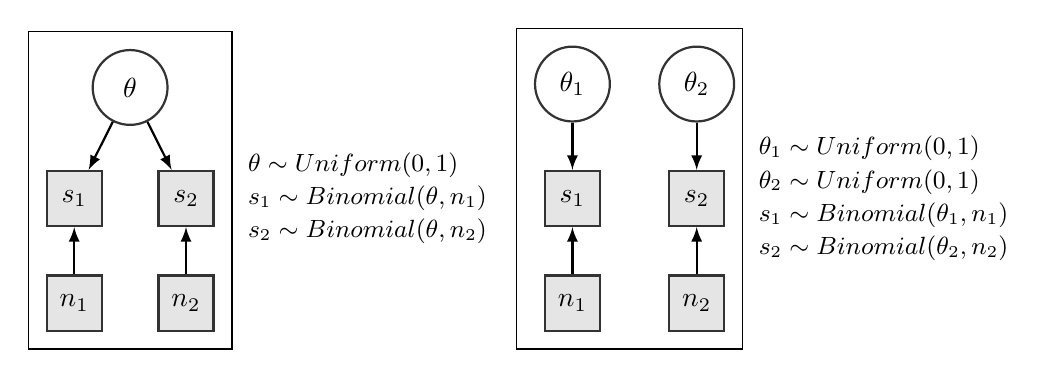
\begin{tikzpicture}
\tikzstyle{main}=[circle, minimum size = 9.5mm, thick, draw =black!80, node distance = 6mm]
\tikzstyle{observed}=[rectangle, minimum size = 7mm, thick, draw =black!80, node distance = 6mm, fill = black!10]
\tikzstyle{connect}=[-latex, thick]
  
  \node[observed] (s1b)  {$s_1$};
   \node[main] (thetab) [above right=7mm and 0mm of s1b] {$\theta$ };
  \node[observed] (s2b) [below right=7mm and 0mm of thetab] {$s_2$};
  \node[observed] (n1b) [below=of s1b] {$n_1$};
  \node[observed] (n2b) [below=of s2b] {$n_2$};
    \path (thetab) edge [connect] (s1b)
        (thetab) edge [connect] (s2b)
        (n1b) edge [connect] (s1b)
        (n2b) edge [connect] (s2b);

  \node[rectangle, inner sep=2.2mm,draw=black!100, fit= (thetab) (n1b) (n2b)] (boxb) {};
  \node[align=left] (textb) [right=3mm of s2b] { \small
$\theta \sim Uniform(0,1)$ \\ \small $s_1 \sim Binomial(\theta, n_1)$ \\ \small $s_2 \sim Binomial(\theta, n_2)$};

\node[observed] (s1) [right=of textb] {$s_1$};
\node[main] (theta1) [above=of s1] {$\theta_1$ };
  \node[main] (theta2) [right=of theta1] {$\theta_2$ };
  \node[observed] (s2) [below=of theta2] {$s_2$};
  \node[observed] (n1) [below=of s1] {$n_1$};
  \node[observed] (n2) [below=of s2] {$n_2$};
  \path (theta1) edge [connect] (s1)
        (theta2) edge [connect] (s2)
             %   (theta1) edge [connect] (theta2)
        (n1) edge [connect] (s1)
        (n2) edge [connect] (s2);
  \node[rectangle, inner sep=2.2mm,draw=black!100, fit= (theta1) (n2)] (box) {};
  \node[align=left] (text) [right=3 mm of s2] {\small
 $\theta_1 \sim Uniform(0,1)$ \\ \small $\theta_2 \sim Uniform(0,1)$ \\ \small $s_1 \sim Binomial(\theta_1, n_1)$ \\ \small $s_2 \sim Binomial(\theta_2, n_2)$};
\end{tikzpicture}
\caption{The generative models used for model comparison. In the left model, the latent variable $\theta$ is the same for both languages whereas in the right model, $\theta$ is different for each of the two languages.}\label{fig:gen-model}
\end{figure}

Returning to my research question, the models corresponding to the \textsc{source hypothesis} and the  \textsc{construction hypothesis} are shown in Figure~\ref{fig:gen-model}. Intuitively, we can imagine the generative process of the data as following. Whenever a child is born, a nurse flips a coin with an unknown probability $\theta$ of landing on head and if the coin lands on head, then the child will use \textit{von} or \textit{from} to mark standards of comparison. In the model on the left, the nurse uses the same coin for all children, whereas in the model on the right, the nurse uses a coin with probability of heads of $\theta_1$ for all German-speaking children and another coin with probability of heads of $\theta_2$ for all English-speaking children. Given the number of German-speaking children who use \textit{von} to mark \textsc{comparison} ($s_1$), the number of English-speaking children who use \textit{from} ($s_2$), and the total number of German-speaking and English-speaking children who use a comparative construction in the corpus ($n_1$ and $n_2$), we can then compute and compare the likelihood of the two models. If it is more likely that the nurse used the same coin, then the data suggest that there is no difference between the two language groups and this would be evidence for the \textsc{Source Hypothesis}. However, if it is more likely that the nurse used two different coins, then the data suggests that there is a difference between the two language groups and this would be evidence for the \textsc{construction hypothesis}.

I implemented these two models in webppl \citep{goodman2014}. I use MCMC as the inference algorithm
and run it with 1,000,000 samples and a burn-in period of 50,000 samples.

\subsection{Results}

Table~\ref{tbl:comp-uses} shows the frequency of utterances with standards of comparison in the German and English corpora. I manually coded all utterances that contain \textit{von}/\textit{from} or \textit{als}/\textit{than} for whether they contain a comparative construction or not\footnote{In order to account for the larger age range of some of the German corpora, I only considered utterances until age 5;0.0.}. There was at least one use of a comparative construction with \textit{als} in all German corpora but no German child produced a comparative construction with \textit{von}. In English, on the other hand, only five children ever expressed \textsc{comparison} and three of them used \textit{from} to mark a standard of comparison. If we run the statistical model from the previous section with these numbers, we get a BF of 4.6, which suggests that significantly fewer German-speaking children use \textit{von} to mark \textsc{comparison} than English-speaking children use \textit{from} for these constructions. 

\begin{table}
\begin{tabularx}{\textwidth}{L{1.7cm} | c  c  c  c  c  c | C{1cm}}
 & Leo & Cosima & Pauline & Sebastian & Caroline & Simone & \\ \hline
Age of & \multirow{2}{*}{2;3} & \multirow{2}{*}{3;10} & \multirow{2}{*}{2;2} & \multirow{2}{*}{3;7} & \multirow{2}{*}{2;7} & \multirow{2}{*}{2;2} & \multirow{2}{*}{2;9} \\
first use & & & & & & & \\  \hline
\textit{von/vom} & 0  & 0  & 0  & 0  & 0  & 0 & 0 \\
\textit{als} & 58  & 1  & 4  & 5  & 11  & 12 & 91 \\ \hline
\textit{von/vom} & \textbf{\texttimes}  & \textbf{\texttimes}  & \textbf{\texttimes}  & \textbf{\texttimes}  & \textbf{\texttimes}  & \textbf{\texttimes} & 0 \\
\textit{als} & \checkmark  & \checkmark  & \checkmark  & \checkmark  & \checkmark  & \checkmark & 6 \\
\end{tabularx}
\addtocounter{table}{-1}

\vspace{1em}
\begin{tabularx}{\textwidth}{L{1.7cm} | C{1.4cm} C{1.2cm}  C{1.2cm}  C{0.75cm}  c  c c  | C{1cm}}
 & Damon & Adam & Sarah &  Eve   & Shem & Abe  & Naomi &  \\ \hline
Age of &  \multirow{2}{*}{2;8^{*}}  &   \multirow{2}{*}{4;2}   &   \multirow{2}{*}{2;10} &   \multirow{2}{*}{2;1} &  \multirow{2}{*}{-}  &  \multirow{2}{*}{3;3} &  \multirow{2}{*}{-}  &  \multirow{2}{*}{3;0} \\  
first use & & & & & & & & \\  \hline
\textit{from} & 18  & 0  & 2  & 0 & 0  & 9  & 0 & 29 \\
\textit{than} & -^{*}  & 21  & 10  & 1 & 0  & 70  & 0 & 102 \\ \hline
\textit{from} &\checkmark  & \textbf{\texttimes}  &\checkmark  & \textbf{\texttimes}  & \textbf{\texttimes}  & \checkmark & \textbf{\texttimes} & 3 \\
\textit{than} & -^{*}  & \checkmark  & \checkmark  & \checkmark  & \textbf{\texttimes}  & \checkmark & \textbf{\texttimes} & 4 \\
\caption{}\label{tbl:comp-uses-en}
\end{tabularx}
\caption{Uses of standards of comparison in the German (top) and English (bottom) corpora. \textit{Age of first use} denotes the age of the first use of a standard of comparison, the numbers in the second and third row show the absolute uses of the respective preposition to mark \textsc{comparison}, and the last two rows indicate whether the child used the respective preposition to mark \textsc{comparison}. The last column shows the average age and the row totals, respectively. *The data for Damon is from \cite{clark1989a}, who only provide the number of utterances with \textsc{comparison} marked with \textit{from} along with several examples.} \label{tbl:comp-uses}
\end{table}

\subsection{Discussion}

The results of this corpus study suggest that only English-speaking children produce standards of comparison that are marked with \textit{from}. This provides evidence for the \textsc{construction hypothesis} as we would not expect a difference between the two languages if these non-conventional productions were independent of the adult input. Further evidence for the \textsc{construction hypothesis} comes from the fact that Sarah and Abe used the conventional comparative \textit{different from} at least once\footnote{\cite{clark1989a} do not mention whether Damon also used this construction at one point.}, which suggests that they picked up this construction from adult uses with \textit{different}.

As shown in Table~\ref{tbl:comp-uses}, Sarah used \textit{from} only twice to mark a standard of comparison. Her first utterance contained the conventional construction \textit{different from} (\textit{dance a different way from us but very nice to see}, 3;10.16). Her second utterance contained \textit{from} in combination with the comparative adjective \textit{higher} (\textit{now the rainbow is gettin(g) higher from the rain}, 5;0.30). However, with this example, it is unclear whether she wanted to express that the height of the rain is a standard of comparison or that the rain causes the rainbow to become higher. Abe, on the other hand, used this construction much more productively with adjectives such as \textit{better}, \textit{longer}, and \textit{same}, and at some point even with the noun \textit{winner} (\textit{[...] I think we're gonna be a winner
from Joey}, 3;8.28). 

Abe shows a lot of consistency in his uses of the two prepositions. He only used \textit{from} to mark \textsc{comparison} until age 3;3 and from then on he exclusively used \textit{than}, with the exception of the example with the noun phrase above. This is consistent with either hypothesis. According to the \textsc{Source Hypothesis}, he would first assume that standards of comparison are a source and then later learn to distinguish them from other arguments. According to the \textsc{construction hypothesis}, one possible developmental path is that he starts with the assumption that \textit{from} marks \textsc{comparison} because of hearing \textit{different from} and later learns that \textit{from} can be used only with one particular adjective.

The adult input is also consistent with the \textsc{construction hypothesis}. All corpora except the Naomi corpus contain at least one adult use of the phrase \textit{different from}\footnote{No input data are available for Damon but considering that \textit{different from } is even more prevalent in British English and considering that his mother is a speaker of British English, it is very likely that he was exposed to this phrase.}, and therefore all children who marked \textsc{comparison} with \textit{from} heard this construction at least once.

Additional evidence for children picking up non-default means of marking \textsc{comparison} from the adult input comes from the German data. As I mentioned in Section~\ref{sec:marking}, German-speaking adults sometimes mark \textsc{comparison} with \textit{wie}, which is prescriptively used only to mark equatives, as well as with \textit{denn}, which is an archaic marker and only being used in a limited number of fixed constructions in modern German. These two prepositions also show up in children's early productions (\ref{ex:simone-comp-denn}-\ref{ex:simone-comp-wie}).
\begin{exe}
\ex \label{ex:simone-comp-denn} \gll aber des is(t) doch bißchen kleiner \textbf{denn} mir, so ein Loper. der is(t) kleiner \textbf{als} mir. \\
but the is after-all a-bit smaller than me such a Loper. the is smaller than me. \\
`But after all, this is a bit smaller than me, such a Loper\footnote{Presumably she is referring to a toy.}. This is smaller than me.' \hfill (Simone; 2;11.18)
\ex \label{ex:simone-comp-wie} \gll größer \textbf{wie} die Giraffe. \\
taller/bigger as the giraffe.\\
`taller as the giraffe.'
\hfill (Simone; 3;01)
\end{exe}
These examples suggest that German-speaking children also pick up non-default means and apply them more liberally than adults would do. 

In summary, the corpus study provides evidence for the \textsc{construction hypothesis}. However, considering the small sample sizes and the fact that children express standards of comparison infrequently, it could also be that German children use \textit{von} to mark \textsc{comparison} but none of these uses were captured on any of the recordings. In order to determine whether the results of the corpus study are consistent with additional data, I conducted an elicitation study, which I describe in the next section.

\section{Elicitation Study}
\label{sec:experiment}

As I mentioned above, children only infrequently express standards of comparison in spontaneous speech and therefore it can be challenging to elicit uses of this construction. One proven method to elicit rare constructions is to ask children to imitate sentences that contain the construction of interest \citep{clark1989b}. When young children are asked to imitate a sentence, they frequently process the sentence through their own linguistic system and produce a version that is closer to what they would have said spontaneously than what they actually heard \citep{slobin1967}. Therefore, if we ask children to imitate a sentence with a standard of comparison marked by \textit{than}, we expect the child to change the preposition to \textit{from} if he or she would also use \textit{from} spontaneously for \textsc{comparison}. At the same time, we can also ask children to imitate ungrammatical sentences with a \textsc{comparison} marked by \textit{from}. If they would spontaneously mark \textsc{comparison} with \textit{from}, then we expect them to imitate the sentence verbatim; otherwise we would expect them to substitute \textit{than} for \textit{from}.

While this method works well for young children up to around age 4;0, older children are a lot better at producing exact imitations \citep{clark1989b} and therefore their imitations are not as much in line with what they would say spontaneously.  However, older children's meta-linguistic abilities also tend to be better and therefore they are better at judging whether a sentence sounds strange and are often capable of fixing an ungrammatical sentence. I therefore asked older children not only to imitate sentences but also to fix each sentence.

Based on the results from the corpus study, I expected children above age 4;6 in both language groups to use the conventional preposition for marking \textsc{comparison} and I did not expect a difference in the rate of use of \textit{from}/\textit{von} for this construction across languages. For children below age 4;6, the two hypotheses make different predictions. According to the \textsc{source hypothesis}, the mean rate of using \textit{von}/\textit{from} to mark \textsc{comparison} should be the same across languages. However, according to the \textsc{construction hypothesis}, young English-speaking children should use \textit{from} more often to mark \textsc{comparison} than German-speaking children use \textit{von}.

\subsection{Subjects}

\begin{table}
\begin{tabularx}{\textwidth}{l | c | c |  c | c | c | c  }
& $n$ & female & male & age range & age mean  & age SD (months) \\ \hline
$<4;6$, ger. &  7  & 3 & 4  & 3;04-4;03  & 3;10 & 3.8 \\
$>4;6$, ger. &  8  & 6 & 2 & 4;09-5;11  & 5;04  & 5.2 \\
$<4;6$, eng. &  9  & 3 & 6 & 2;08-4;02  & 3;07 & 6.1 \\
$>4;6$, eng. & 11 & 4 & 7 & 4;06-6;01  & 5;04 & 7.3 \\
\end{tabularx}
\caption{Sex and age statistics of subjects in each age and language group.}\label{tbl:subjects}
\end{table}

The subjects were 17 children acquiring Austrian German and 20 children acquiring American English. The German-speaking children were recruited and tested at the KIWI Alterlaa nursery school in Vienna, Austria, and the English-speaking children were recruited and tested at the Bing nursery school in Stanford, CA. All children were growing up in monolingual households but some of the English-speaking children had Spanish-speaking nannies. I excluded two German-speaking children from my analyses (one boy aged 2;7.4 and one girl aged 3;9.29) as they omitted arguments or responded with completely different sentences more than 80\% of the time. I grouped the remaining children into two age groups: younger than 4;6 and older than 4;6. Table~\ref{tbl:subjects} shows sex and age statistics for the two age groups in each language. The German and English subject groups slightly differ in two respects. First, the age range of the younger English-speaking group is larger than the one of the younger German-speaking group as almost all children at the nursery school in Vienna were older than 3;6, and second, the sex distribution varies across languages. While both differences could potentially be problematic, the results from the corpus study do not suggest that there are  any differences by sex. Further, all children who used \textit{from} to mark \textsc{comparison} continued to do so up until at least age 3;8, which is older than several of the German-speaking subjects in my sample.

\subsection{Procedure}

I tested each English-speaking child in a small game room with a table and chairs outside the classroom. Before each session, I put a set of 22 cards, a pig puppet, and a sheet of paper with five colored circles on the table. I took each child into the room and introduced him or her to the pig puppet with the sentences ``So, this is Oscar.  And do you know what Oscar really likes? When you always say whatever he says. So, for example, if Oscar says \textit{Hello}. What do you say then?'', using a different voice for \textit{Hello}. Most children then replied with ``Hello'' and otherwise I encouraged them to say ``Hello'' by saying ``Can you also say \textit{Hello}?''. I then said the more complex sentence ``\textit{I am a pig with pink ears}.'' in Oscar's voice and again, if children did not immediately imitate, I encouraged them again by saying ``Can you also say \textit{I am a pig with pink ears}?''. Once the child imitated the more complex utterance, I said ``\textit{The cards are under the table}.'' in Oscar's voice while the cards were on the table,  and I encouraged the child again to repeat what Oscar said. Most children imitated the semantically incorrect utterance verbatim but some noticed right away that something was wrong with the utterance. If the child imitated verbatim, I followed up with ``But wait, the cards are actually not under the table, no. Oscar sure says silly things sometimes. Can you help him say it better?'' and repeated variants of the question ``Can you help him say it better?'' until the child responded with ``The cards are on (top of) the table''. If the child noticed a problem with the utterance right away, I responded with ``You are right, the cards are not under the table. Oscar sure says silly things sometimes. Can you help him say it better?''.

After this training session, I explained to the child that we were going to play a short game and explained that the child should draw a card and then Oscar would say a sentence about the card and that the child should say whatever Oscar says. I further explained that after five cards, the child would get a golden star sticker, which he or she could put on the sheet of paper in front of him or her.

The actual session proceeded then as follows. I asked the child to turn over the first card in the pile. Each card contained either a drawing of a child or a drawing or photo of an object (see Appendix~A for the pictures), which corresponded to the subject of a stimulus. I then introduced the person or object on the card with ``Oh, that's `NAME{'}'' or ``Oh, the `OBJECT{'}'' in my voice and then said the sentence associated with the person or the object in Oscar's voice. When the child did not immediately imitate, I said ``Can you also say \textunderscore\textunderscore\textunderscore\textunderscore\textunderscore \ ?'' until the child produced an \textsc{imitation}. For the youngest children (aged 3;8 and below\footnote{I originally intended to set the cutoff at 3;5 as \cite{clark1989b} did. However, some of the children between 3;5 and 3;8 did not produce any repairs and therefore I ended up using a higher cutoff.}), I only asked them to imitate what Oscar said;  the other children were also asked whether they could ``say it better'' to elicit the \textsc{repair}. This procedure was repeated for each of the 22 cards in randomized order. Some of the children were very reluctant to produce repairs and if they repeatedly refused to ``say it better'', I reminded them that Oscar sometimes says silly things and that he needs their help.

I recorded all sessions using the Voice Memos app on an iPhone 6.

The procedure for the German children was identical to the described procedure with the exception that a) I used a puppet of the snowman ``Olaf'' from the Disney movie ``Frozen''\footnote{I intended to use the same puppet at Bing but the research staff recommended that I use something more neutral because ``Frozen'' is more popular among children in the US than in other countries and they were worried that using a character from the movie might be too distracting for the children.} and b) I tested the children in a corner of the classroom instead of in a separate room. The German script that I used at the beginning of each session is in Appendix~C.

\subsection{Materials}

\begin{table}
\begin{tabularx}{\textwidth}{L{8.5cm} | l}
\multicolumn{2}{ l }{\textbf{Grammatical sentences}} \\ \midrule
(8) Olivia went home from school & \multirow{2}{*} {locative source}   \\
(11) Jacob brought in sand from outside &  \\ \hline
(1) Anna got bitten by a large crocodile & \multirow{2}{*} {agent} \\
(4) The monkeys were fed by the children & \\ \hline
(5) The mouse is smaller than the bear & \multirow{2}{*} {standard of comparison} \\
(6) The elephant is heavier than the rabbit &  \\ \hline
(10) Mia played with Emma & \multirow{2}{*} {accompaniment} \\
(13) Hans built a tower with his dad &  \\ \hline
(14) Sophia caught a duck with her hands & \multirow{2}{*} {instrument} \\
(19) James ate the soup with a big spoon &  \\ \hline
(15) Noah drank the milk from the bottle & \multirow{2}{*} {filler} \\
(17) The flowers are from the garden &  \\ \bottomrule
\end{tabularx}

\vspace{1em}
\begin{tabularx}{\textwidth}{L{8.5cm} | l}
\multicolumn{2}{ l }{\textbf{Ungrammatical sentences}} \\ \midrule
(18) The strawberries are with the farm &  {locative source}   \\
(22) The bus went with Palo Alto to Stanford &  (\textit{with} \textrightarrow \ \textit{from})  \\ \hline
(3) The dog was petted with grandma &  {agent} \\
(12) Lisa was tickled with her mom &  (\textit{with} \textrightarrow \ \textit{by}) \\  \hline
(7) The plane is faster from the train &  {standard of comparison} \\
(9) The horse is bigger from the frog & (\textit{from} \textrightarrow \ \textit{than})  \\ \hline
(2) The cat cuddled from her mom & {accompaniment} \\
(20) Elsa danced from Dan &  (\textit{from} \textrightarrow \ \textit{with}) \\ \hline
(16) Emma cut an apple from a knife &  {instrument} \\
(21) Ben can fix his toy from a hammer &  (\textit{from} \textrightarrow \ \textit{with}) \\ \bottomrule
\end{tabularx}
\caption{Sentences used in the English elicitation task. The number in front of each sentence denotes the number on the corresponding card in Appendix~{A}. The expected substitutions for the ungrammatical sentences are shown below each category.} \label{tbl:materials-en}
\end{table}

I tested each child with 22 sentences. Four sentences contained a locative source, four a demoted agent, four a standard of comparison, four an accompanier, and four an instrument\footnote{For the question whether German-speaking children mark standards of comparison with \textit{von}, only the four sentences with a standard of comparison are relevant, and all the other items can be seen as fillers. However, I discuss some of the other results in Section~\ref{sec:agents-possessors}.}. Half of the sentences were grammatical and half of them were ungrammatical because they contained a wrong preposition. The remaining two sentences contained a locative source, conventionally marked with \textit{from} in English, and with \textit{aus} (\textit{out of}) in German; these served as fillers to balance the number of prepositions and the number of sentences with \textit{from} that children heard in each language. The English and German sentences were translations of each other with two exceptions. First, I localized the names with the exception of the names of three ``Frozen'' characters. For both languages, I only used names or common nicknames of names that were among the 20 most common names for newborns in 2014 in Austria\footnote{http://www.statistik.at/web{\_}de/statistiken/menschen{\_}und{\_}gesellschaft/ bevoelkerung/geborene/haeufigste{\_}vornamen/index.html} and the US\footnote{https://www.ssa.gov/oact/babynames/}, respectively.  Second, instead of a translation of the English sentence *\textit{The bus went with Palo Alto to Stanford}, I used a German translation of the sentence *\textit{The train went with Vienna to Graz} to localize the town names and to give a realistic means of transportation. The list of English sentences is in Table~\ref{tbl:materials-en} and the German sentences are in Appendix~{B}.

The cards corresponding to the sentences always showed the subject of the sentence. While in theory, the cards were not necessary for the task, their use provided several advantages. First, they made the sentences sound less out of context. By first introducing the person or object on the card, it seemed more natural that the puppet would say something about the person or object as compared to the puppet uttering the sentences out of the blue. Second, for the sentences with names in subject position, the cards provided me with a way to make sure that the children understood that the subject was a person, even if they had not heard that name before. Third, the cards provided a context in which it was natural to promote a patient to subject position as the person on the card became the topic of the conversation. Finally, since the children liked the cards, they made the task more interesting for them.


\subsection{Coding}

I transcribed all the recordings and then manually coded each of the responses. My main goal was to determine from the responses whether a child would use the conventional (adult-like) preposition for a certain argument.

For the \textsc{imitation} responses, I used three coding categories: \textsc{correct}, \textsc{incorrect}, and \textsc{other}. \textsc{correct} and \textsc{incorrect} responses expressed the correct verb and all its arguments, whereas \textsc{other} responses either omitted some arguments or responded with a completely different sentence. \textsc{correct} responses contained the target preposition whereas \textsc{incorrect} responses contained a different preposition. In general, I considered responses with a verb form different from the one in the stimulus (i.e., different in tense or person) as \textsc{correct} or \textsc{incorrect} unless the child had changed the response from passive to active or vice versa. For example, I counted substituting \textit{was building} for \textit{built} as \textsc{correct} or \textsc{incorrect}, depending on which preposition was used, but I counted substituting  \textit{was tickling} for \textit{was tickled} as \textsc{other}. Substituting names, substituting pronouns for noun phrases, swapping the order of noun phrases in comparative constructions, substituting or omitting determiners, and adding or omitting modifiers did not affect the coding decision.

Considering that children provided free form responses and that they interpreted the task in different ways, I elicited some responses that demonstrated their ability to use the right preposition but that would have been coded as \textsc{other} according to my guidelines. These included omitting the sentence-final German auxiliary \textit{werden} (`become') as well as responding with utterances that only contained an oblique noun phrase, as in  ``\textit{No, with a fork}''. I coded these responses as \textsc{correct} or \textsc{incorrect}. For the ungrammatical sentences with locative sources, many children changed the preposition to a locative preposition other than \textit{from} (e.g., \textit{the strawberries are at the farm}). As these changes made the sentence grammatical but did not demonstrate whether a child knew how to express locative sources, I coded such responses as \textsc{other}.   

For the \textsc{repair} responses, I used the same categories as well as a fourth category, \textsc{no response}, for when a child did not produce a \textsc{repair} response.

Some children frequently made changes to the sentence when I asked them to imitate, but then either repeated what they said before or did not respond to my request for a \textsc{repair} response;  other children first imitated verbatim and then changed the preposition in their \textsc{repair} response. To make it easier to compare results, I therefore also combined the \textsc{imitation} and \textsc{repair} responses. Generally, I only considered the better response\footnote{``Better'' in this context means to be ranked higher according to the ordering \textsc{correct} $>$ \textsc{incorrect} $>$ \textsc{other} $>$ \textsc{no response}.} of the two responses unless the child imitated a grammatical sentence verbatim and then substituted a different preposition such that the response became ungrammatical. I considered these cases \textsc{incorrect}. For the youngest children who only provided imitations, the \textsc{combined} responses are only determined by (and therefore identical to) their \textsc{imitation} responses.

%Apart from coding each response individually, I also considered the entire transcripts and noted for each child whether he or she substituted at least once  \textit{than}/\textit{als} with \textit{from}/\textit{von}  and whether he or she substituted at least once \textit{from}/\textit{von} marking a SoC with \textit{than}/\textit{als}.

\subsection{Results and Discussion}




While German and English are very similar in many respects, there are also notable differences between the two languages. For example, German has a more complex case system, is more flexible in terms of word order, and has a more complex gender system than English. All these differences could potentially make the task harder for children in one of the two language groups and therefore invalidate any comparison across languages. Before discussing my results, I therefore first consider whether there were any unexpected differences across the two language groups.



There was no significant difference in how often German- and English-speaking children were able to produce exact imitations of the stimulus sentences in either age group (younger age group: German 49\%, English 61\%, BF=1.2; older age group: German 66\%, English 69\%, BF=0.14). %run_test(76, 120 , 154, 198, 0.5) and run_test(116, 176, 168, 242, 0.5)
Second, and more important, if we consider the \textsc{combined} responses and look at how often children made a relevant change to a sentence according to the coding criteria, there was again no significant difference across the two languages (younger age group: German 30\%, English 25\%, BF=0.18; older age group: German 24\%, 
English 27\%, BF=0.25). %run_test(46, 51 , 153, 198, 0.5) and run_test(42, 66 , 176, 242, 0.5)
The latter result suggests that children in both language groups were equally likely to change a preposition or change an entire sentence, which indicates that children in both language groups were able to perform the task equally well. However, there was one difference between the older German-speaking children and the older English-speaking children: The German-speaking children refused to provide \textsc{repair} responses significantly more often than the English-speaking children (German 74\%, English 34\%, BF$>$10E13). This implies that the \textsc{combined} responses for the older German-speaking group are significantly more often only determined by their \textsc{imitation} responses. Considering that older children tend to be better at imitating sentences verbatim, this difference makes comparisons in terms of how well the older children in both language groups were able to correct ungrammatical sentences  problematic because a lower performance by the German-speaking group might solely reflect less willingness to cooperate rather than a lower proficiency\footnote{I believe there were two reasons for the lower rate of \textsc{repair} responses by the German-speaking children. First, as I was testing the German-speaking children in the classroom, they were more distracted than the English-speaking children, and second, the English-speaking children at BING were much more used to participating in experiments and most likely felt more comfortable doing the task than the German-speaking children did.}. For the younger children, there was no significant difference between the two language groups. Overall,  these results suggest that the findings from the German and the English data are comparable with the exception of the \textsc{repair} and \textsc{combined} responses to ungrammatical sentences in the older age group.

%Children in both language groups made a relevant change more often to ungrammatical sentences than to grammatical ones (German: grammatical 8\%, ungrammatical 49\%, BF$>$10E14; English: grammatical 12\%, ungrammatical 45\%, BF$>$10E12). This result shows that children notice the wrong preposition in the ungrammatical sentences and change these sentences according to what they believe is right.



\begin{table}
\begin{tabularx}{\textwidth}{l | c   c  c |  c   c  c  }
\multicolumn{7}{l}{\textbf{Grammatical sentences}}\\ \midrule
& \multicolumn{3}{c | }{Younger children} & \multicolumn{3}{c}{Older children} \\
& \textsc{correct} & \textsc{incorr.} & \textsc{other} & \textsc{correct} & \textsc{incorr.} & \textsc{other} \\ \hline
German & 88 & 0 & 12 & 95 & 2 & 3 \\
English & 84 & 5 & 11 & 92 & 4 & 5 \\ \midrule
\multicolumn{7}{l}{\textbf{Ungrammatical sentences}}\\ \midrule
& \multicolumn{3}{c | }{Younger children} & \multicolumn{3}{c}{Older children} \\
& \textsc{correct} & \textsc{incorr.} & \textsc{other} & \textsc{correct} & \textsc{incorr.} & \textsc{other} \\  \hline
German & 41 & 49 & 10 & 43 & 54 & 4 \\
English & 27 & 63 & 10 & 41 & 52 & 7 \\
\end{tabularx}

\caption{Relative frequencies (\%) of types of responses to all grammatical and ungrammatical sentences. The responses are the result of combining the \textsc{imitation} and \textsc{repair} responses as described above.}\label{tbl:res-gramm-ungramm}
\end{table}

\begin{figure}
\includegraphics[width=0.5\textwidth]{graphs/gramm-ungramm-younger.pdf} \includegraphics[width=0.5\textwidth]{graphs/gramm-ungramm-older.pdf} 
\caption{Relative frequencies of types of responses to all grammatical and ungrammatical sentences by younger children (left) and older children (right). The responses are the result of combining the \textsc{imitation} and \textsc{repair} responses as described above.}\label{fig:gramm-ungramm}
\end{figure}


The overall results are presented in Figure~\ref{fig:gramm-ungramm} and Table~\ref{tbl:res-gramm-ungramm}. The two plots show the relative frequencies of types of responses to grammatical and ungrammatical sentences for each language and age group. In all age and language groups, the relative frequency of \textsc{correct} responses to ungrammatical stimuli was significantly above 0 (BF$>$10E6 for all groups), which again shows that children are not merely imitating the stimuli or making random changes but instead providing sensible corrections, either in their \textsc{imitation} or in their \textsc{repair} responses.

Figure~\ref{fig:gramm-ungramm} also suggests that English-speaking children in the younger age group were worse at correcting ungrammatical sentences than German-speaking children in the same age group. The primary reason for this difference is that English-speaking children were worse for sentences with \textsc{comparison} and demoted agents. While this difference was not significant (BF=1.23), it was very consistent for all stimuli with these two constructions, which suggests that this difference could be significant given a larger sample size.

\begin{figure}
\includegraphics[width=0.5\textwidth]{graphs/comparison-responses-younger.pdf} \includegraphics[width=0.5\textwidth]{graphs/comparison-responses-older.pdf} 
\caption{Relative frequencies of types of responses to grammatical and ungrammatical sentences with standards of comparison by younger children (left) and older children (right). The responses are the result of combining the \textsc{imitation} and \textsc{repair} responses as described above.}\label{fig:soc-items}
\end{figure}

Figure~\ref{fig:soc-items} shows the relative frequencies of responses to the stimuli with \textsc{comparison}. Qualitatively,  German-speaking children in the younger age group were better at correcting sentences with \textit{von} marking \textsc{comparison} than English-speaking children in the same age group. Further, only English-speaking children changed grammatical sentences to ungrammatical ones; all of them did so by substituting \textit{from} for \textit{than}. In the older age group, again only English-speaking children changed grammatical sentences. At the same time, older English-speaking children also appeared to be better at substituting \textit{than} for \textit{from} in response to ungrammatical stimuli. Quantitatively, none of these differences were significant. However this is likely a result of the small sample size; notice that these results are very consistent with the corpus results. The only surprising difference is the lower rate of correct responses to the ungrammatical stimuli by the older German-speaking children. This is probably the outcome of the low repair rate in this group, which I mentioned above.

\begin{figure}
\hspace{0.25\textwidth}\includegraphics[width=0.5\textwidth]{graphs/non-imit-uses-comp-from.pdf}
\caption{Relative frequencies of children within the younger (left) and older (right) age group who at least once substituted  \textit{from}/\textit{von} for \textit{than}/\textit{als}.}\label{fig:soc-children}
\end{figure}

Instead of considering individual responses, we can also consider the entire transcript in a manner similar to that applied to the corpus study. Figure~\ref{fig:soc-children} shows the fraction of children within each age group and language who at least once substituted \textit{from}/\textit{von} for \textit{than}/\textit{als}.  Thirty-three percent of the younger English-speaking children made such a substitution whereas none of the German-speaking children did so. If we incorporate the prior from the corpus study, younger English-speaking children mark \textsc{comparison} significantly more often with \textsc{from} (BF=6.32). Among the older children, only one English-speaking child substituted \textit{from} for \textit{than} and the difference between German- and English-speaking children within the older age group was not significant (BF=0.2).

These results are consistent with the results of the corpus study and provide further evidence for the \textsc{construction hypothesis}. There is a clear difference between early marking of \textsc{comparison} in German and English, which can be easily explained by the differences in the input. The \textsc{source hypothesis}, on the other hand, does not offer an explanation for this difference; both languages express locative source with a preposition and if some English-speaking children use \textit{from} to mark \textsc{comparison} because they perceive the standard of comparison as a source, then some German-speaking children should show a similar behavior. 

From a qualitative point of view, the results of the elicitation task further highlight the importance of the adult input. One German-speaking child (F;3.11.0) substituted \textit{wie}, the equative-marking preposition, for \textit{von}. As I mentioned earlier, \textit{wie} is used by some adults to mark \textsc{comparison}.


I conclude from the results of the corpus study and the elicitation task that English-speaking children most likely overextend the construction \textit{different from} rather than relying on a conceptual category of \textsc{source} when they mark \textsc{comparison} with \textit{from}. However, this conclusion raises another question: Why do comparative constructions with \textit{different} play such a prominent role?  Several other adjectives such as \textit{good}, \textit{big}, \textit{nice}, and \textit{old} appear much more frequently in the adult input and therefore it seems surprising that the construction \textit{different from} has a significant impact on children's early marking of standards of comparison. However, this becomes less surprising if we consider only comparative adjectives with an explicitly expressed standard of comparison because the construction \textit{different from} is among the most frequent comparative constructions in the adult input. Table~\ref{tbl:adjectives} shows the frequencies of adjectives that appear at least 5 times in comparative constructions in the combined adult input of the corpora from the previous section. As this table shows, despite the fact that the adjective \textit{different} appears overall much less frequently than \textit{big} or \textit{good},  the construction \textit{different from} is  among the most frequent comparative constructions. This table also shows that adults rarely express standards of comparisons in child-directed speech; note that these numbers are the total uses in 6 longitudinal corpora. This observation suggests that on the one hand, a small number of adult utterances with \textit{different from} could have a significant impact on a child's acquisition of comparative constructions, and on the other hand, it suggests that if a child assumes that \textit{from} can be used to mark \textsc{comparison}, it might take him or her a long time to acquire the conventional means as he or she receives little input that contradicts the child's hypothesis.

\begin{table}
\begin{tabularx}{\textwidth}{l | c  | c | c |  c  | c | c | c  }
 & big & good & old & different & bad & tall & small \\ \midrule
Overall frequency & 1,407 & 2,493 & 338 & 190 & 263 & 78 & 173 \\ \hline
Comparative  & \multirow{2}{*}{32} & \multirow{2}{*}{27} & \multirow{2}{*}{12} & 9 (\textit{from})& \multirow{2}{*}{9} & \multirow{2}{*}{8} & \multirow{2}{*}{5}  \\
constructions &      &      &      &   3 (\textit{than})  & & &  \\
\end{tabularx}
\caption{Overall frequency and frequency of comparative constructions with an explicit standard of comparison for several adjectives in the English adult input, summed across the corpora from Section~\ref{sec:corpus}.  These are all the adjectives that appear at least 5 times in a comparative construction with a standard of comparison in the adult input.}\label{tbl:adjectives}
\end{table}

%ungrammatical sentences > 0:
%younger EN: run_test(0, 24, 90, 90, 0.5) ; BF>10E6
%younger DE: run_test(0, 29, 70, 70, 0.5) ; BF>10E8
%older EN: run_test(0, 45, 110, 110, 0.5); BF>10E14
%older DE: run_test(0, 34, 80, 80, 0.5); BF> 10E10

%ungrammatical sentences younger DE vs younger EN:
%run_test(24, 29, 90, 70, 0.5); BF = 1.23




%EXACT IMITATIONS

%ENGLISH

%- younger children imitate less often exactly than older ones, but not significantly (61\% vs. 69\%, BF=0.71)
% R command: run_test(120, 168, 198, 242, 0.5)

%- no difference with regards to grammatical/ungrammatical sentences (gr. 66\%, ungr. 65\%, BF=0.12)
% run_test(159, 129, 240, 200, 0.5)


%GERMAN

%- younger children produce exact imitations significantly less often than older ones (younger 49\%, older 66\% BF=13.6)

%run_test(76, 116 , 154, 176, 0.5)

%- no difference between grammatical and ungrammatical (grammatical: 68\%, ungrammatical: 66\%, BF=0.22)

% run_test(122, 116 , 170, 150, 0.5)

%GERMAN VS. ENGLISH

%- no difference between German and English ( German: 58\%, English: 65\% BF=0.71)

% run_test(288, 192 , 440, 330, 0.5)

%no difference for younger (German: 49\%, English: 61\%, BF=1.2)

%run_test(76, 120 , 154, 198, 0.5)


%no difference for older (German: 66\%, English: 69\%, BF=0.14)

%run_test(116, 176, 168, 242, 0.5)

%========

%CHANGES

%ENGLISH

%- children change ungrammatical sentences significantly more often (either by changing the preposition or by changing the entire sentence) (BF>10e12, 12\%, gr. 45\%)
% run_test(28, 89, 240, 200, 0.5)

%- no age difference (younger make as many changes as older ones) (25\% younger, 27\% older, BF=0.12)
%run_test(51, 66, 198, 242, 0.5)

%GERMAN

%- children change ungrammatical sentences significantly more often (either by changing the preposition or by changing the entire sentence) (BF>10e14, 8\%, gr. 49\% ungr)

%run_test(15, 73, 180, 150, 0.5)

%- no age difference (30\% younger, 24\% older, BF=0.27) 

% run_test(46, 42, 154, 176, 0.5)

%GERMAN VS. ENGLISH

%younger ones: no significant differences in changes (25\% (en), 30\% (de), BF=0.18)

%run_test(46, 51 , 153, 198, 0.5)


%older ones: no significant differences in changes (27\% (en), 24\% (de), BF= 0.15)
% run_test(42, 66 , 176, 242, 0.5)



\section{Demoted Agents and Possessors}
\label{sec:agents-possessors}

In the previous two sections, I argued that the non-conventional uses of \textit{from} to mark \textsc{comparison} are most likely not a result of children perceiving the prepositional complement as a {source}. However, my account does not provide an explanation for the non-conventional marking of demoted agents or possessors, which \cite{clark1989a,clark1989b} observed in corpora and -- in the case of demoted agents --  in an elicitation task. Considering that German-speaking children as well as adults also use \textit{von} to mark possessors and demoted agents, all the data are compatible with the following \textsc{revised source} account.

\begin{quote}
Children perceive temporal sources, demoted agents, causes, natural forces, and possessors (but not standards of comparison) as a source and therefore mark all of these arguments with the preposition \textit{from} or the equivalent marker of locative sources in other languages.
\end{quote}

However, there are some observations that while not contradicting the \textsc{revised source} account, raise the question whether it is the best explanation for the data. First, if we assume a relationship between conceptual categories and language typology, then the \textsc{revised source} category seems very unlikely. There are only three languages in a sample of 98 languages that show the case syncretism of \textsc{revised source}: German (using \textit{von}), Middle English (\textit{of(f)}), and Old Spanish (\textit{de}) \citep{palancar2002}. If \textsc{revised source} was a prominent and universal conceptual category, we might assume that more languages could express all these arguments with the same means.

Second, \cite{clark1989a} argue that all English-speaking children first assign the meaning of a locative source to \textit{from} based on the fact that the first utterance with \textit{from} of all investigated children expressed a locative source, and they argue that the non-conventional uses are an overextension of the locative meaning. However, this is not the case for German-speaking children. Only two of them marked a locative source in their first utterance with \textit{von}, whereas the other four either marked a possessor or used a partitive construction.

Third, the \textsc{revised source} account no longer assumes that children assign only one meaning to \textit{from} but rather that some children assume that \textit{from} marks \textsc{source} as well as \textsc{comparison}. While children might still initially assume that \textit{from} is monosemous and can only be used to mark \textsc{source}, some children start to use \textit{from} to mark \textsc{comparison} before age 3 and from that point on they must assume that \textit{from} is polysemous. This is per se not problematic but once we abandon the assumption that children assign only one meaning to \textit{from}, there is no reason to believe that children cannot assign three or more meanings to \textit{from}.

Fourth, possessors and demoted agents vastly differ in frequency -- both in the adult input and in early productions. Demoted agents are rare in spoken language whereas possessors are very frequent. Nevertheless, English-speaking children use \textit{from} approximately as often to mark demoted agents as they use it to mark possessors. At the same time, they use \textit{'s} and \textit{of} two orders of magnitude more often than they use \textit{from} to mark possessors. 

All of these observations suggest that there might be a better explanation for the non-conventional uses of \textit{from} for demoted agents and possessors. I discuss these types of arguments in detail in turn.

\subsection{Demoted agents}

\begin{figure}
\hspace{0.25\textwidth}\includegraphics[width=0.5\textwidth]{graphs/non-imit-uses-agent-from.pdf}
\caption{Relative frequencies of English-speaking children within the younger (left) and older (right) age group who at least once marked an agent with \textit{from}.}\label{fig:agt-children}
\end{figure}

The use of \textit{from} for demoted agents in English appears to be the most consistent non-conventional use of \textit{from}. In my elicitation task, I was able to reproduce the results by \cite{clark1989b}. Figure~\ref{fig:agt-children} shows the relative frequency of children who marked agents with \textit{from} for both age groups. Forty-four percent of the younger children and 36\% of the older children used \textit{from} at least once to mark an agent despite the fact that all of the stimuli with demoted agents marked them using either \textit{by} or \textit{with}. The relative frequencies in both age groups are significantly greater than 0 (younger age group: BF=4.66, older age group: BF=3.54).

These non-conventional uses are particularly interesting because adults only infrequently use demoted agents in conversational speech and for this reason, demoted agents are virtually non-existent in the input. On average, adult utterances with a demoted agent appeared only 9 times within each corpus and this number already includes several out-of-context uses in the Adam, Eve, and Sarah corpora to test whether the child was able to understand passive constructions. Considering that children rarely hear demoted agents marked with \textit{by}, it is therefore not surprising that children do not know the conventional means to express demoted agents. Nevertheless, the lack of input does not explain why children consistently opt for \textit{from}.

One explanation for this behavior is provided by the \textsc{revised source} account. \cite{clark1989a} argued that children perceive agents as the source of an event and therefore mark demoted agents using the preposition that is used to mark locative sources. However, there are two other possible explanations, which do not assume that children make abstract overgeneralizations. 

First, it could be that some children perceive demoted agents as a cause and therefore mark them with \textit{from}. Some evidence for this hypothesis comes from the typological literature. In the sample of 98 languages by \cite{palancar2002}, 46 languages from a large variety of families mark demoted agents and causes using the same means. This suggests that this case syncretism developed independently, which in return might suggest that there could be  a cognitive basis for perceiving demoted agents as causes. 
 Further evidence comes from the findings that children tend to use adjectival \textit{get}-passives before regular passives \citep{borer1987,fox1998}, which could suggest the following developmental path. Children first acquire the conventional construction \textit{get ADJ from CAUSE} and then overextend this construction to the non-conventional \textit{get PARTICIPLE from AGENT} and \textit{be PARTICIPLE from AGENT} before realizing that the conventional construction is \textit{be/get PARTICIPLE by AGENT}. None of the English corpora that I investigated are dense enough to confirm or disprove this developmental path, but some children did produce utterances with the construction \textit{get ADJ from CAUSE} at an early age (e.g., \textit{Who gets sick from eating seeds?}, Abe, 3;1.8), and all other constructions appeared in some responses to the elicitation task.

Second, it could be that children overextend the use of \textit{from} to mark natural forces. While this also appears to be a plausible overextension, this hypothesis is very unlikely to be true given the fact this construction appears even less frequent in the adult input than demoted agents. Further, apart from Damon, only Sarah used \textit{from} to mark a natural force and she did so after she had begun to mark agents with \textit{from}.

It could also be that children take all these constructions as evidence that agents should be marked with \textit{from}. The two hypotheses do not contradict each other and therefore it could be that all of these constructions contribute to children's assumptions on how agents should be marked.  

All of this is speculative at this point, and I do not have additional evidence for either hypothesis. However, there seems to be as much evidence that children perceive demoted agents as causes, as there is that they perceive demoted agents as sources. Further, both of my explanations assume that less abstraction is required of the child and therefore I argue that they should be considered in future work on this topic.

\subsection{Possessors and Partitives}

\begin{table}
\hspace{0.125\textwidth}\begin{tabularx}{0.75\textwidth}{l | c | c | c | c | c | c }
& Adam & Sarah &  Eve   & Shem & Abe  & Naomi  \\ \midrule
\textit{'s} & 272 &   179 & 60 &   203 & 446 &  184 \\
\textit{of} & 592 & 268 & 70 & 160 & 782 & 79 \\
\textit{from} & 0 & 1 & 0 & 5 & 7 & 0 \\
\end{tabularx}
\caption{Frequencies of possessive \textit{'s}, \textit{of}, and \textit{from} used to mark possessors.}\label{tbl:poss}
\end{table}


The phenomenon that children mark possessors with \textit{from} appears to be quite distinct from the non-conventional expression of demoted agents for several reasons. First, exchange and possession are among the earliest and most frequent topics of conversation of young children across many different cultures (e.g., \cite{stern1928,brown1973,tomasello1998}). Second, children know the conventional means of expressing possession: All children who marked possessors with \textit{from} expressed possession with the clitic \textit{'s} or the preposition \textit{of} at least two orders of magnitude more often than they did with \textit{from} (see Table~\ref{tbl:poss}) and all children talked about possession before or at the same time as they produced their first utterance with \textit{from} to mark a locative source. Children at any age therefore clearly do not assume that \textit{from} is the primary device to mark possessors but at most that it can be used along with \textit{'s} and \textit{of}. 

Some of the non-conventional uses appear to be overextensions of conventional constructions. For example, Shem produced the utterance \textit{dat's [that's] a finger from him} (3;0.13) a few days after he uttered \textit{dat's [that's] from my -- um -- puppet show} (3;0.5, talking about a lion puppet). Both utterances express a part-of relation between two objects: The puppet is a part of the puppet show  and the finger is part of the person that Shem is talking about. However, the construction \textit{that's NP1 from NP2} can only be used when NP1 can be physically detached from NP2, which makes \textit{that's a finger from him} ungrammatical. This difference might not be completely apparent to a three-year-old child and it is likely that he overextended the conventional construction.

Other non-conventional uses such as \textit{I see boats from mommy} (Adam, 3;0.0) or \textit{you can be a mom from two babies} (Damon, 3;7.5) are harder to explain based on conventional constructions and they might be rooted in non-linguistic conceptual difficulties. Despite the fact that children talk a lot about possession, they have difficulty in determining ownership of objects up until at least age 5. \cite{friedman2008} ran a study that showed that children up until age 5 have a strong bias towards assigning ownership of a toy to whoever interacted with it first. This bias persists to a large extent even if the person who first interacted with the toy gives the toy to another person and the child is being told that the second person got the toy as a present. This bias can only be overcome if the presentation is made more prototypical by wrapping the toy and not letting the first person interact with it. It is therefore conceivable that children misinterpret frequent adult utterances such as \textit{That's a present from Granny Hart} (Mother to Eve, 1;9) to mean that the grandmother still owns the toy rather than that the child got the toy from the grandmother. If children misinterpret such utterances, then it would not be surprising if they occasionally used \textit{from} to mark possessors.

These explanations are again speculative but they again illustrate that there exist reasonable explanations that do not assume that children perceive possessors as an abstract source.

\section{Conclusion and Future Directions}

In this paper, I revisited the phenomenon that English-speaking children use the preposition \textit{from} for more types of arguments than adults. I compared how English- and German-speaking children express standards of comparison in a corpus study as well as an elicitation experiment, and I argued on the basis of the results from these two studies that the non-conventional uses of \textit{from} to mark standards of comparison are the result of overextending the conventional construction \textit{different from}, one comparative form that children hear from early on.

I also discussed the uses of \textit{from} to mark demoted agents as well as possessors and presented new explanations for both phenomena that do not assume that children can make very abstract generalizations. These explanations, however, are only speculative at this point and more work is needed to determine whether any of these possibilities are superior to the \textsc{revised source} account. One possible avenue to test some of these hypotheses would be to investigate the use of prepositions in other languages with different case syncretisms. In Italian, for example, adults mark demoted agents with the source-marking preposition \textit{da} but they mark causes and possessors with \textit{di}. Therefore, the presence or absence of consistent non-conventional uses of either preposition could provide new insights on why English-speaking children mark demoted agents with \textit{from}.

To conclude, I argued for an explanation of some of the non-conventional uses of \textit{from} that does not assume that children rely on an abstract conceptual category in formulating their utterances. While this work clearly falls short of being a comprehensive account of the acquisition of grammatical prepositions, it demonstrates the complexity of this process and shows that future research in this area should focus more on specific constructions in different languages rather than only focusing on what all non-conventional uses of a grammatical preposition have in common.

%=====================================================================

\bibliography{qp-references}

\section*{Appendix A: Pictures for Elicitation Study}

\includegraphics[page=1, width=\textwidth]{pictures/pictures-v3-all.pdf}

\includegraphics[page=2, width=\textwidth]{pictures/pictures-v3-all.pdf}

\includegraphics[page=3, width=\textwidth]{pictures/pictures-v3-all.pdf}

\includegraphics[page=4, width=\textwidth]{pictures/pictures-v3-all.pdf}

\pagebreak

\section*{Appendix B: German Stimuli}\begin{table}[h!]
\begin{tabularx}{\textwidth}{L{10.2cm} | l}
\multicolumn{2}{ l }{\textbf{Grammatical sentences}} \\ \midrule
(8) Sarah ist von der Schule nachhause gegangen & \multirow{2}{*} {locative source}   \\
(11) Tim hat den Sand von draußen mitgebracht &  \\ \hline
(1) Anna ist von einem großen Krokodil gebissen worden & \multirow{2}{*} {agent} \\
(4) Die Affen sind von den Kindern gefüttert worden & \\ \hline
(5) Die Maus ist kleiner als der Bär & \multirow{2}{*} {comparison} \\
(6) Der Elefant ist schwerer als der Hase &  \\ \hline
(10) Mia hat mit Emma gespielt & \multirow{2}{*} {accompaniment} \\
(13) Hans hat mit seinem Papa einen Turm gebaut &  \\ \hline
(14) Marie hat eine Ente mit ihren Händen gefangen & \multirow{2}{*} {instrument} \\
(19) Max hat die Suppe mit einem großen Löffel gegessen &  \\ \hline
(15) Lukas hat die Milch aus der Flasche getrunken & \multirow{2}{*} {filler} \\
(17) Die Blumen sind aus dem Garten &  \\ \bottomrule
\end{tabularx}

\vspace{1em}
\begin{tabularx}{\textwidth}{L{10.2cm} | l}
\multicolumn{2}{ l }{\textbf{Ungrammatical sentences}} \\ \midrule
(18) Die Erdbeeren sind mit dem Bauernhof &  {locative source}   \\
(22) Der Zug ist mit Wien nach Linz gefahren & (\textit{mit} \textrightarrow \ \textit{von}) \\ \hline
(3) Der Hund ist mit Oma gestreichelt worden &  {agent} \\
(12) Lisa ist mit ihrer Mama gekitzelt worden &   (\textit{mit} \textrightarrow \ \textit{von}) \\ \hline
(7) Das Flugzeug ist schneller von dem Zug &  {comparison} \\
(9) Das Pferd ist größer von dem Frosch &  (\textit{von} \textrightarrow \ \textit{als}) \\ \hline
(2) Die Katze hat von ihrer Mama gekuschelt & {accompaniment} \\
(20) Elsa hat von Elias getanzt &  (\textit{von} \textrightarrow \ \textit{mit}) \\ \hline
(16) Julia hat einen Apfel von einem Messer geschnitten &  {instrument} \\
(21) Felix kann sein Spielzeug von einem Hammer reparieren &  (\textit{von} \textrightarrow \ \textit{mit}) \\ \bottomrule
\end{tabularx}
\caption{Sentences used in the German elicitation task. The number in front of each sentence denotes the number on the corresponding card in Appendix~{A}.} \label{tbl:materials-en}
\end{table}

\pagebreak

\section*{Appendix C: German Script}

(Passages in \textit{italics} were uttered in ``the puppet's'' voice.)

\vspace{1.0em}

\noindent \textbf{E(xperimenter)}: Das is Olaf! Weißt du was Olaf ganz gerne mag? Wenn man immer genau das sagt, was er sagt. Also wenn er sagt ``\textit{Hallo}'', kannst du dann auch ``Hallo'' sagen?

\vspace{0.5em}

\noindent \textbf{C(hild):} Hallo

\vspace{0.5em}

\noindent \textbf{E}: \textit{Ich habe eine Karotte als Nase.}

\vspace{0.5em}

\noindent \textbf{C}: Ich habe eine Karotte als Nase.

\vspace{0.5em}

\noindent \textbf{E}: \textit{Die Karten liegen unter dem Tisch.}

\vspace{0.5em}


\noindent \textbf{C}: Die Karten liegen unter dem Tisch.

\vspace{0.5em}


\noindent \textbf{E}: Aber das stimmt ja gar nicht, oder? Der Olaf sagt manchmal dumme Sachen. Kannst du ihm helfen das besser zu sagen?

\vspace{0.5em}

\noindent \textbf{C}: Die Karten liegen auf dem Tisch.


%=====================================================================

%\begin{addresses}
 % \begin{address}
%    Author1 \\
%    Street \\
%    \ldots \\
%    \email{author1@email}
%  \end{address}
%  \begin{address}
 %   Author2 \\
 %   Street \\
 %   \ldots \\
 %   \email{author2@email}
 % \end{address}
 % ...
%\end{addresses}

%=====================================================================

\end{document}
